% Final presentation (10-15 min + Q&A). Build: make (slides PDF and speaker-notes PDF).
\documentclass[aspectratio=169,10pt]{beamer}
% shared preamble for the final presentation and the class talk
\usetheme[progressbar=frametitle,numbering=fraction]{metropolis}
\usepackage[T1]{fontenc}
\usepackage{booktabs,tabularx,array,xcolor,tikz,pgfpages,listings}
\usetikzlibrary{arrows.meta,positioning,fit,calc,shapes.geometric}
\definecolor{ink}{HTML}{17262B}\definecolor{acc}{HTML}{1F5FAD}\definecolor{ok}{HTML}{2E7D32}
\definecolor{warn}{HTML}{D9822B}\definecolor{pale}{HTML}{EEF3F8}
\setbeamercolor{frametitle}{bg=ink}
\setbeamercolor{progress bar}{fg=acc}
\setbeamercolor{alerted text}{fg=acc}
\setbeamertemplate{note page}[plain]
\usepackage{xspace}
\newcommand{\pg}{PostgreSQL\xspace}
\newcolumntype{L}[1]{>{\raggedright\arraybackslash}p{#1}}
\newcolumntype{Y}{>{\raggedright\arraybackslash}X}
\newcommand{\ok}[1]{\textcolor{ok}{\textbf{#1}}}
\newcommand{\wa}[1]{\textcolor{warn}{\textbf{#1}}}
\tikzset{
  box/.style={draw=acc,rounded corners=2pt,align=center,fill=pale,font=\scriptsize,minimum height=9mm,text width=22mm},
  io/.style={draw=gray,align=center,fill=gray!10,font=\scriptsize,minimum height=8mm,text width=19mm},
  orc/.style={draw=ok,rounded corners=2pt,align=center,fill=ok!8,font=\scriptsize,minimum height=7mm,text width=22mm},
  fl/.style={-{Stealth[length=1.6mm]},thick,draw=ink},
  bk/.style={-{Stealth[length=1.6mm]},dashed,draw=acc}}

\ifdefined\shownotes\setbeameroption{show only notes}\fi
\title{Grammar-Aware Fuzzing of PostgreSQL\\with Typed Derivation Trees, and Beyond}
\subtitle{CS-5187 Software Analysis, Term Project A3 \quad final presentation}
\author{Venu Kummari \and Bhuvan Chilukuti \and Gowtham Reddy}
\institute{IIT Guwahati}
\date{November 2026}

\begin{document}

\maketitle
\note{VENU. We built a dynamic-analysis tool, a fuzzer, for PostgreSQL that looks for wrong
results, not only crashes, and then generalized it to four more SQL engines. We will spend most
of the time on how the tool works and how it found its bugs: nine PostgreSQL bugs reported, seven
fixed upstream, five with our patches; three more fixes filed to DuckDB, Turso and DataFusion.}

\begin{frame}{The problem: bugs that do not crash}
\begin{columns}[T]
\column{0.55\textwidth}
\begin{itemize}
  \item Target: \textbf{\pg}, the most used open-source database; its planner changes weekly.
  \item Worst bug class: a \textbf{wrong result}: no error, no crash, no log line.
  \item Crash fuzzers (SQLsmith, Squirrel) cannot see it; SQLancer finds it with small hand-written generators.
  \item Both need a \textbf{test oracle}: how do we know the right answer?
\end{itemize}
\column{0.42\textwidth}
\begin{block}{Our answer}
Generate SQL as \alert{typed derivation trees} and turn each tree into
\alert{checks that know the answer}: equivalent queries, other plans, the last release.
\end{block}
\end{columns}
\end{frame}
\note{VENU. The software-analysis question is the oracle problem. A fuzzer can run millions of
queries, but it must decide automatically whether an answer is wrong. Our tool decides by
comparison: the same question asked in a different but equivalent way must give the same answer.}

\begin{frame}{Outline}
\begin{enumerate}
  \item \textbf{Arbor}, the \pg fuzzer: architecture and five techniques
  \item Evaluation and \textbf{how the tool found each bug}
  \item The \textbf{generalized fuzzer}: DuckDB, SQLite, Turso, DataFusion
  \item Team, limitations, conclusion
\end{enumerate}
\end{frame}
\note{VENU. Three parts: the PostgreSQL fuzzer, how its bugs were found, and the generalization.}

\section{Arbor: the PostgreSQL fuzzer}

\begin{frame}{Architecture}
\centering\resizebox{\linewidth}{!}{% architecture of the PostgreSQL fuzzer
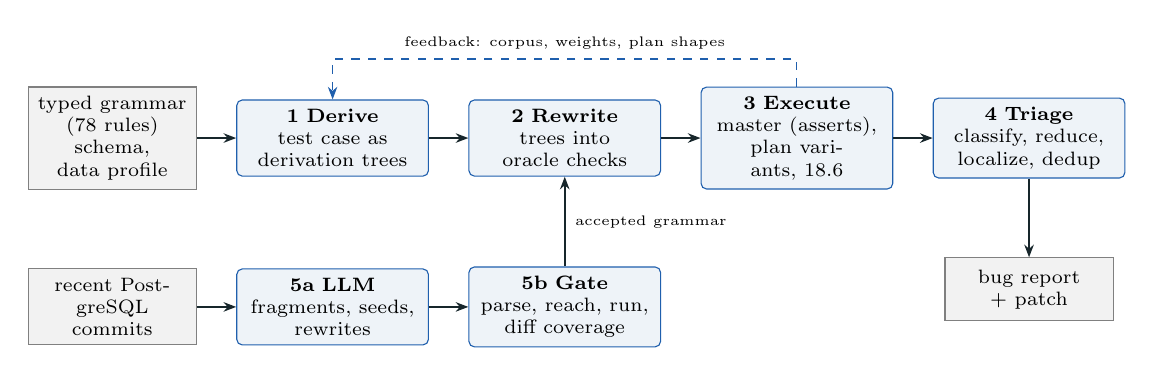
\begin{tikzpicture}[node distance=4mm and 5mm]
\node[io] (g) {typed grammar (78 rules)\\schema, data profile};
\node[box,right=of g] (s1) {\textbf{1 Derive}\\test case as\\derivation trees};
\node[box,right=of s1] (s2) {\textbf{2 Rewrite}\\trees into\\oracle checks};
\node[box,right=of s2] (s3) {\textbf{3 Execute}\\master (asserts),\\plan variants, 18.6};
\node[box,right=of s3] (s4) {\textbf{4 Triage}\\classify, reduce,\\localize, dedup};
\node[io,below=10mm of g] (c) {recent \pg commits};
\node[box,right=of c] (l1) {\textbf{5a LLM}\\fragments, seeds,\\rewrites};
\node[box,right=of l1] (l2) {\textbf{5b Gate}\\parse, reach, run,\\diff coverage};
\node[io,below=10mm of s4] (r) {bug report\\+ patch};
\draw[fl] (g)--(s1); \draw[fl] (s1)--(s2); \draw[fl] (s2)--(s3); \draw[fl] (s3)--(s4); \draw[fl] (s4)--(r);
\draw[bk] (s3.north) -- ++(0,0.35) -| node[pos=0.25,above,font=\tiny]{feedback: corpus, weights, plan shapes} (s1.north);
\draw[fl] (c)--(l1); \draw[fl] (l1)--(l2); \draw[fl] (l2.north) -- node[right,font=\tiny]{accepted grammar} (s2.south -| l2.north);
\end{tikzpicture}
}
\small
\begin{itemize}
  \item Python, about 10{,}500 lines, 151 unit tests; one worker per server, savepoints isolate test cases.
  \item The derivation tree is used four times: \alert{generate, mutate, rewrite into oracles, reduce}.
\end{itemize}
\end{frame}
\note{VENU. Top row: the fuzzing loop. Step 1 derives a test case from the typed grammar as
derivation trees. Step 2 rewrites the trees into oracle checks. Step 3 runs everything on master
built with assertions, under other planner settings, and on release 18.6. Step 4 classifies,
reduces and localizes failures. Bottom row: the LLM loop extends the grammar from recent commits,
but only what passes a gate on the real server. Feedback (new plan shapes, new outcomes) goes back
into the corpus and the weights.}

\begin{frame}[fragile]{Technique 1: a typed grammar that produces trees}
\begin{columns}[T]
\column{0.5\textwidth}
\small
\begin{itemize}
  \item Own DSL (\texttt{.pgg}): 78 rules, 421 alternatives, 13 SQL types; types are parameters (\texttt{expr<T>}).
  \item Scope-aware: names, aliases, column types bound while deriving $\Rightarrow$ \alert{99.3\%} of statements valid (random mutation: 26\%).
  \item Each test case is kept as trees; \textbf{replay} re-derives a tree after an edit and re-binds names.
  \item Feedback: corpus of novel test cases, subtree mutation, bandit weights per alternative, data-profile literals near real values.
\end{itemize}
\column{0.47\textwidth}
\begin{lstlisting}[basicstyle=\ttfamily\scriptsize]
expr<T:num> : expr<T> "+" expr<T>
            | <0.5> ABS "(" expr<T> ")"
            | @col(T) | @lit(T) ;
pred : expr<T> cmp expr<T>
     | expr<T> IS NOT? NULL ;
\end{lstlisting}
\scriptsize Types make every subtree replaceable by another subtree of the same type: the basis of the rewrites and of reduction.
\end{columns}
\end{frame}
\note{GOWTHAM. The grammar is our own format. Every expression carries its SQL type, so whatever
we generate type-checks, and the server spends its time on planning and executing, not on
rejecting syntax. Keeping the tree lets us replace any subtree with another of the same type,
which the next three techniques use. Bandit weights raise alternatives that led to new plan shapes;
the data profile picks literals near the values in the tables, so predicates select some rows.}

\begin{frame}{Technique 2: the oracle stack}
\small
\begin{tabularx}{\linewidth}{@{}lXl@{}}
\toprule
Oracle & What is compared or detected & Bug class \\
\midrule
crash / assertion & backend dies; assertion text from the server log & crash \\
internal error & SQLSTATE \texttt{XX000} (``should not happen'') & internal error \\
hang & query outlives \texttt{statement\_timeout} and cancel & hang \\
plan variants & same query under 18 planner settings (join methods, parallel, \dots) & wrong result \\
metamorphic & query vs. its \alert{tree rewrite}: TLP, NoREC, expression, predicate & wrong result \\
cross-version & master vs. release 18.6, same database & regression \\
CERT & adding a restriction must not raise the row estimate & bad estimate \\
RLS & row-level security must hide the same rows as a filter & data leak \\
\bottomrule
\end{tabularx}

\medskip
Determinism filter: only statements whose results may be compared (no \texttt{LIMIT} without total order, no clock functions); floats masked once per check.
\end{frame}
\note{BHUVAN. Eight oracles, each catching a different class. The first three only watch the
server. The other five compare two answers that must agree. A plan variant changes how PostgreSQL
runs a query, never what it returns. Cross-version compares master with the last release.
Comparisons are only made where they are sound: we skip non-deterministic queries.}

\begin{frame}{Technique 3: metamorphic rewrites on the tree}
\begin{columns}[T]
\column{0.52\textwidth}
\small
\textbf{TLP} (ternary logic partitioning): pick a predicate $p$ in the tree, then
\[ Q \;=\; Q_{p} \uplus Q_{\neg p} \uplus Q_{p\ \mathrm{IS\ NULL}} \]
\textbf{NoREC}: the filter moved into the select list must count the same rows.

\textbf{Expression rewrites}: $e \rightarrow (\mathrm{SELECT}\ e)$, $e+0$, \dots{} for a typed subtree.
\column{0.45\textwidth}
\small
\begin{itemize}
  \item Applied at \alert{any query level} (subqueries, CTEs), because the tree tells where a predicate is and what type it has.
  \item A mismatch is \textbf{confirmed} by re-running both sides before it is reported.
  \item 12 rewrite kinds; each was checked on live runs for false positives.
\end{itemize}
\end{columns}
\end{frame}
\note{BHUVAN. A string rewriter does not know where a predicate starts or what type an expression
has. On the tree both are known, so the rewrite is type-correct at any nesting level. For example,
wrapping an expression in a sub-select must not change its value; it does change what the planner
can simplify, which is exactly what found one of our bugs.}

\begin{frame}{Technique 4: triage, from a failure to a report}
\small
\begin{columns}[T]
\column{0.5\textwidth}
\begin{enumerate}
  \item \textbf{Reproduce} 3 times on a fresh server (else flaky).
  \item \textbf{Reduce}, three levels:
    \begin{itemize}
      \item tree: replace a subtree by the \alert{smallest derivation of the same rule and type}, replay;
      \item statement delta debugging (ddmin);
      \item token hierarchical delta debugging.
    \end{itemize}
  \item \textbf{Localize}: which plan variant, rewrite or version flips it.
  \item \textbf{Deduplicate} by signature (outcome, culprit, stack frames).
\end{enumerate}
\column{0.46\textwidth}
\begin{block}{Why the tree helps}
Token reduction gets stuck when removing any token breaks the SQL. Tree reduction keeps every candidate valid: \textbf{116 $\rightarrow$ 79 tokens} on a real case.
\end{block}
\begin{itemize}
  \item Verdict ledger: 93 candidates, every one decided.
  \item Git bisection script for regressions.
\end{itemize}
\end{columns}
\end{frame}
\note{BHUVAN. Triage turns a raw failure into something a maintainer will read. The tree
reduction is the fourth use of the tree: it shrinks by replacing subtrees with minimal ones and
replays, so the candidate stays valid SQL and the server's time is spent only on the question
whether the failure remains. Localization tells us which planner setting or which rewrite matters,
which points at the faulty code.}

\begin{frame}{Technique 5: the LLM proposes, the server decides}
\small
\begin{columns}[T]
\column{0.48\textwidth}
\begin{enumerate}
  \item \textbf{Mine} recent planner/executor commits (+ their regression tests).
  \item \textbf{Prompt}: commit diff + grammar excerpt $\rightarrow$ grammar \alert{fragment}, seed tests, rewrite templates.
  \item Every prompt and response stored; replay is deterministic and free.
\end{enumerate}
\column{0.48\textwidth}
\begin{block}{Validation gate (on the server)}
\begin{enumerate}
  \item parses with the grammar, known builtins only
  \item reachable: derived in $\geq 5$ of 150 samples
  \item $\geq 60\%$ of its statements run
  \item seeds run
  \item executes more of the commit's \alert{changed lines} (gcov diff coverage)
\end{enumerate}
Rewrites also need a value probe + 150 live checks.
\end{block}
\end{columns}
\end{frame}
\note{GOWTHAM. The LLM reads a recent commit and proposes grammar for the feature it touches. We
never trust it: a fragment enters the fuzzer only if PostgreSQL accepts what it generates and it
actually executes the lines the commit changed, measured with gcov. In our runs 4 of 10 commits
passed. Our lesson: a tested rewrite is not a proven one; one accepted rewrite changed a collation.}

\section{Evaluation and how the bugs were found}

\begin{frame}{Evaluation setup and results}
\small
Base: master \texttt{26bd08fb} with assertions; reference 18.6; \textbf{5 trials $\times$ 1 h} per arm; Mann--Whitney U, Vargha--Delaney $\hat A_{12}$.

\medskip
\begin{tabularx}{\linewidth}{@{}lX@{}}
\toprule
RQ & Result \\
\midrule
RQ1 reach & valid statements 99.3\% vs 26.0\% (random); backend lines \textbf{36.7\% vs 22.2\%} ($\hat A_{12}=1.00$, $p=0.008$); oracles: plan shapes $\times1.7$ \\
RQ2 bugs & 93 candidates: 8 real, 15 duplicates of real bugs, 42 false positives (all classes fixed), 28 flaky \\
RQ3 benchmark & 23 real fixes reverted in one build; best arm found 2 of 20 in 1 h $\Rightarrow$ 1 h is short \\
RQ4 LLM & +5 SQL features ($p=0.004$), no coverage gain; 4 of 10 commits pass the gate \\
\bottomrule
\end{tabularx}

\medskip
Lesson: \alert{oracle precision}, not generator reach, limits a wrong-result fuzzer.
\end{frame}
\note{GOWTHAM. RQ1: typing pays, valid queries reach far more backend code. RQ2: the oracles find
real bugs, but false positives were the main cost; we fixed every class we found. RQ3 is our ground
truth: we re-injected 23 real bugs, and one hour per trial finds few. RQ4: the LLM adds features,
not coverage.}

\begin{frame}{How the tool found the \pg bugs}
\scriptsize
\begin{tabularx}{\linewidth}{@{}L{0.16\linewidth}L{0.2\linewidth}Yl@{}}
\toprule
Bug type & Technique that found it & How the signal appeared & Upstream \\
\midrule
assertion (parallel plans) & LLM fragment + TLP check & assertion fired while running the TLP check of an LLM-derived query; text taken from the server log & \ok{fixed} \#19803 \\
wrong output (formatting) & cross-version oracle & master and 18.6 printed different strings for the same call & \ok{fixed, our patch} \#19771 \\
assertion (statistics) & extended-statistics clause generator & random statistics objects + clauses reusing their expressions & \ok{fixed, our patch} \\
assertion / wrong result & grammar fuzzer, then cross-version & assertion on master; 18.6 gave a silently wrong answer & \ok{fixed, our patch} \#19768 \\
wrong result (anti-join) & cross-version + TLP & master returned a row that 18.6 and the partition sum did not & \ok{fixed, our patch} \\
hang & hang oracle & query outlived the timeout and ignored cancel & \ok{fixed, our patch} \\
internal error & internal-error oracle (\texttt{XX000}) & grammar arm, \texttt{MERGE} on partitioned tables & \ok{fixed} \#19802 \\
wrong result (constant folding) & expression rewrite $e\rightarrow(\mathrm{SELECT}\ e)$ & the sub-select blocked a planner simplification; results differed & \wa{open} \#19793 \\
bad estimate & CERT oracle & a restriction raised the row estimate (1000 $\rightarrow 10^{100}$) & \wa{open} (patch) \\
\bottomrule
\end{tabularx}
\end{frame}
\note{GOWTHAM and BHUVAN share this slide. Read across: each bug was found by a specific
technique. Two came only from comparing versions; one only from the sub-select rewrite, which
changes what the planner may simplify; one only from the hang oracle; one only from the estimate
oracle. That is the point of having a stack of oracles. Every one of them is rediscovered by the
tool in one 150-second run.}

\begin{frame}{From signal to accepted fix: one pipeline for every bug}
\centering
\resizebox{\linewidth}{!}{%
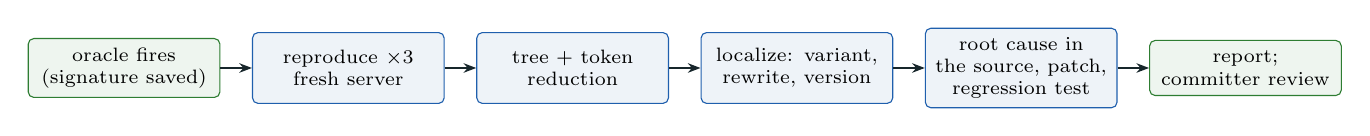
\begin{tikzpicture}[node distance=3mm and 4mm]
\node[orc] (a) {oracle fires\\(signature saved)};
\node[box,right=of a] (b) {reproduce $\times3$\\fresh server};
\node[box,right=of b] (c) {tree + token\\reduction};
\node[box,right=of c] (d) {localize: variant,\\rewrite, version};
\node[box,right=of d] (e) {root cause in\\the source, patch,\\regression test};
\node[orc,right=of e] (f) {report;\\committer review};
\draw[fl] (a)--(b); \draw[fl] (b)--(c); \draw[fl] (c)--(d); \draw[fl] (d)--(e); \draw[fl] (e)--(f);
\end{tikzpicture}}

\medskip
\small
\begin{itemize}
  \item Example: the cross-version oracle flagged a difference; reduction left one function call; localization: ``version''; the root cause: the string terminator was copied into the output; our patch was committed.
  \item \textbf{Result: 9 reported, 7 fixed upstream (5 with our patches), 2 under review with our patches.}
  \item One command reproduces the headline: \texttt{sudo bash scripts/reproduce.sh} $\Rightarrow$ ``Known bugs reproduced: 9 of 9''.
\end{itemize}
\end{frame}
\note{VENU. Every bug went through the same steps; only the first box differs. The tool does
everything up to localization automatically; root cause and patch are our work, and maintainers
committed five of our patches.}

\section{The generalized fuzzer}

\begin{frame}{Beyond \pg: architecture}
\centering\resizebox{!}{0.62\textheight}{% architecture of the generalized fuzzer
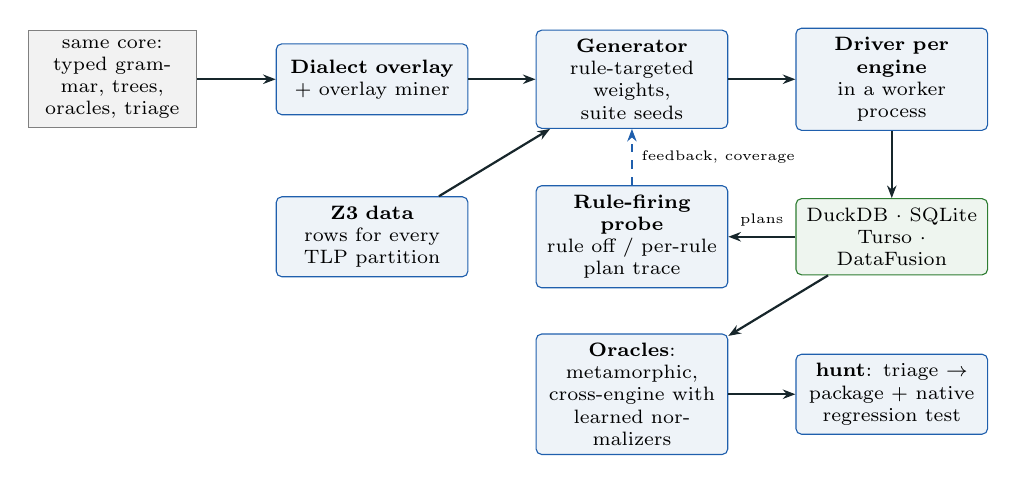
\begin{tikzpicture}
\node[io]  (core) at (0,0)     {same core: typed grammar, trees, oracles, triage};
\node[box] (ov)   at (3.3,0)   {\textbf{Dialect overlay}\\+ overlay miner};
\node[box] (gen)  at (6.6,0)   {\textbf{Generator}\\rule-targeted weights,\\suite seeds};
\node[box] (drv)  at (9.9,0)   {\textbf{Driver per engine}\\in a worker process};
\node[box] (z3)   at (3.3,-2)  {\textbf{Z3 data}\\rows for every\\TLP partition};
\node[box] (rule) at (6.6,-2)  {\textbf{Rule-firing probe}\\rule off / per-rule\\plan trace};
\node[orc] (eng)  at (9.9,-2)  {DuckDB $\cdot$ SQLite\\Turso $\cdot$ DataFusion};
\node[box] (orc)  at (6.6,-4)  {\textbf{Oracles}: metamorphic,\\cross-engine with\\learned normalizers};
\node[box] (hunt) at (9.9,-4)  {\textbf{hunt}: triage $\rightarrow$\\package + native\\regression test};
\draw[fl] (core)--(ov); \draw[fl] (ov)--(gen); \draw[fl] (gen)--(drv); \draw[fl] (drv)--(eng);
\draw[fl] (z3)--(gen);
\draw[fl] (eng)--node[above,font=\tiny]{plans}(rule);
\draw[bk] (rule)--node[right,font=\tiny]{feedback, coverage}(gen);
\draw[fl] (eng)--(orc); \draw[fl] (orc)--(hunt);
\end{tikzpicture}
}
\small
\begin{itemize}
  \item Same trees and oracles; new: drivers, overlays, rule firing, Z3 data, learned normalizers, autonomous loop.
  \item Branch \texttt{generalized}, 192 unit tests.
\end{itemize}
\end{frame}
\note{VENU. The PostgreSQL fuzzer is tied to PostgreSQL in three places: the executor, the
grammar and the planner settings. Each became an interface: a driver per engine in its own worker
process, a dialect overlay on the same grammar, and optimizer-rule switches. Everything else, the
trees, oracles and triage, is reused unchanged.}

\begin{frame}{Generalized techniques (1): engines, overlays, rule firing}
\small
\begin{columns}[T]
\column{0.5\textwidth}
\textbf{Engine abstraction}: \texttt{Driver} (execute, error classes, rules, plans) in a spawned worker: a crash or Rust panic kills only the worker.

\medskip
\textbf{Dialect overlays}: \texttt{\%drop}, \texttt{\%replace}, \texttt{\%droptype} with cascade over the \pg grammar.
\textbf{Overlay miner}: alternatives that almost never execute become \texttt{\%drop} lines: DuckDB \textbf{32\% $\rightarrow$ 44\%} valid with no manual line.

\medskip
Valid queries with overlays: DuckDB 96.3\%, SQLite 97.7\%, Turso 93.3\%, DataFusion 79.4\%.
\column{0.47\textwidth}
\textbf{Optimizer-rule firing} replaces code coverage:
\begin{itemize}
  \item rule fires $\Leftrightarrow$ plan changes when the rule is switched off;
  \item SQLite: 30 switches via \texttt{sqlite3\_test\_control} (found in the symbol table); DuckDB: \texttt{disabled\_optimizers}; DataFusion: \texttt{EXPLAIN VERBOSE} shows each rule's effect;
  \item uses: feedback (new rules/pairs), coverage metric, \alert{rule-targeted generation}, localization;
  \item ground truth: SQLite gcov build, 69.4\% of optimizer lines from 200 cases.
\end{itemize}
\end{columns}
\end{frame}
\note{VENU. Rule firing is our engine-independent feedback: it needs no instrumented build and
it is about the optimizer, where logic bugs live. For SQLite we call a test-control function that
the Python binding does not export, by finding its address in the symbol table.}

\begin{frame}{Generalized techniques (2): data, comparison, autonomy}
\small
\begin{itemize}
  \item \textbf{Z3 data synthesis}: the predicate subtree (comparisons, \texttt{AND/OR/NOT}, NULL logic, \texttt{BETWEEN}, \texttt{IN}, \texttt{LIKE}) becomes constraints; Z3 yields rows so every TLP partition is non-empty (non-vacuous checks 34\% $\rightarrow$ 40\%, first version).
  \item \textbf{Learned normalizers}: probe two engines with small typed queries, cluster disagreements, pick normalizers (float digits, \texttt{2.0}/\texttt{2}, booleans) and guards: DuckDB vs SQLite disagreements \textbf{28.7\% $\rightarrow$ 3.6\%}.
  \item \textbf{Test suites as seeds}: sqllogictest and Turso tests imported (DataFusion: 406 files, 19{,}602 statements, 83\% run).
  \item \textbf{Autonomous loop} \texttt{pgfuzz hunt}: campaign $\rightarrow$ triage $\rightarrow$ package with a regression test \alert{in the engine's own format} (\texttt{.test}, \texttt{.slt}, \texttt{.sqltest}).
\end{itemize}
\end{frame}
\note{BHUVAN. Data synthesis attacks vacuous checks: a TLP check proves nothing if the table has
no rows for some partition. Normalizers make two different engines comparable without hand-written
rules. The hunt loop runs the whole pipeline without us and drafts the package we file.}

\begin{frame}{How the generalized fuzzer found its bugs}
\scriptsize
\begin{tabularx}{\linewidth}{@{}L{0.09\linewidth}L{0.16\linewidth}YL{0.2\linewidth}@{}}
\toprule
Engine & Bug type & How it was found & State \\
\midrule
Turso & wrong result / spurious error & Turso-vs-SQLite differential oracle; reduced to one aggregate call; root cause: arguments read from non-consecutive registers & \wa{filed with fix} \#11594 / PR \#11595 \\
DuckDB & internal error (2.0.0 regression) & internal-error oracle on the nightly build; a regression since 2.0.0; root cause: the binder copies an expression that cannot be copied & \ok{approved by a maintainer} \#28551 / PR \#28552 \\
DataFusion & internal error in DML & internal-error oracle; root cause: common-subexpression elimination leaks a plan-only column into DML planning & \wa{filed with fix} \#27235 / PR \#27236 \\
DataFusion & internal error (planning order) & internal-error oracle & fix ready \\
Turso & panic / spurious error & worker caught a Rust panic; reduced to an aggregate in \texttt{IN (SELECT ...)} next to a window function; still on the newest \texttt{main} & fix ready \\
Turso, DuckDB & panic, rejected join, bind error & worker caught a Rust panic / error; bisection on \texttt{main} & fixed upstream before we filed \\
\bottomrule
\end{tabularx}

\medskip
\small Every filed fix has a regression test in the engine's own format and passes the engine's full test suite (e.g.\ 12{,}700 Turso tests, all 546 DataFusion sqllogictest files).
\end{frame}
\note{GOWTHAM. Same pipeline as for PostgreSQL. The Turso bug was found only by comparing with
SQLite; the others by the internal-error oracle. Before filing, we re-checked each one on the
engine's newest code built from source; three had already been fixed, which we found by
bisection. The three filed pull requests are open and awaiting review.}

\section{Wrap-up}

\begin{frame}{Who did what}
\small
\begin{columns}[T]
\column{0.32\textwidth}
\textbf{Venu Kummari}
\begin{itemize}
  \item tool design and implementation: grammar, oracles, triage, LLM gate, benchmark
  \item paper; \#19768, \#19793
  \item generalized fuzzer and its 3 fixes
\end{itemize}
\column{0.32\textwidth}
\textbf{Bhuvan Chilukuti}
\begin{itemize}
  \item RQ3 benchmark campaign
  \item bug hunts on recent features
  \item patches: NOT IN, IGNORE NULLS, statistics, MCV
\end{itemize}
\column{0.32\textwidth}
\textbf{Gowtham Reddy}
\begin{itemize}
  \item server builds, RQ1/RQ2/RQ4 campaigns
  \item LLM arm (10 commits)
  \item \#19802, \#19803; \texttt{to\_char} fix
\end{itemize}
\end{columns}
\medskip
\small Signed statement in the paper; commit history shows the same split. Each of us can explain every part.
\end{frame}
\note{EACH MEMBER says one sentence about their part.}

\begin{frame}{Limitations and future work}
\small
\begin{itemize}
  \item 5 trials per arm: effect sizes rather than always significance; false-positive fixes not re-measured by a new campaign.
  \item One schema, one commit for \pg; LLM: free-tier model on ten commits.
  \item Generalized: evaluation runs (rule feedback, Z3, normalizers, SQLancer baseline, DuckDB benchmark) are scripted and dry-run tested; the full runs take about four days.
  \item DataFusion validity (79\%) below the 95\% of the other engines.
\end{itemize}
\end{frame}
\note{VENU. We state plainly what the results do not show.}

\begin{frame}{Conclusion}
\begin{columns}[T]
\column{0.24\textwidth}\centering{\Huge\textbf{9}}\\\small \pg bugs reported
\column{0.24\textwidth}\centering{\Huge\ok{7}}\\\small fixed upstream (5 our patches)
\column{0.24\textwidth}\centering{\Huge\textbf{3}}\\\small more fixes filed (DuckDB, Turso, DataFusion)
\column{0.24\textwidth}\centering{\Huge\textbf{36.7\%}}\\\small backend lines (random 22.2\%)
\end{columns}
\bigskip
\begin{block}{Take-away}
Valid SQL is the easy part; knowing the right answer is the hard part. Typed trees make sound
rewrites possible, measured precision shows where an oracle is still wrong, and the same core
carries over to other engines.
\end{block}
\end{frame}
\note{VENU. Close with the numbers and the take-away.}

\begin{frame}[standout]
Thank you. Questions?\\[6pt]
\normalsize github.com/PASS-IITG/cs5187-term-project-blazing-bhuvi\\
\small generalized: github.com/v28k/cs5187-term-project (branch \texttt{generalized})
\end{frame}

\end{document}
